% !TeX root = ../../thesis.tex
\chapter{Introduction}\label{ch:introduction}
This chapter presents an overview of non-valence anions, focusing on dipole-bound anions (DBAs). The significance of these anions in biological systems is explored, followed by an introduction to biological quinones and their crucial role in biological processes. Finally, the research objectives are outlined.

\section{Non-Valence Anions}
An anion is an atom or molecule possessing one or more excess electrons. The binding of an additional electron to a neutral molecule is a balance between the attractive potential between the excess electron and the nuclei, and the repulsive forces from the neutral molecule's electrons. Unlike valence electrons in neutral species, these "extra" electrons do not experience a -1/r Coulombic attraction at long distances. Instead, they interact through weaker charge-multipole potentials, which are less robust than the covalent bonds holding the molecule together \cite{simons2008molecular, herbert2015quantum}.

The binding energy of the excess electron is typically significantly lower than the ionisation energy of the neutral molecule, leading to changes ranging from geometry relaxation to chemical reactions with surrounding species. In discussions of molecular anions, the concept of electron affinity (EA) is key. The adiabatic electron affinity (AEA) quantifies the energy difference between a molecule and its corresponding anion, both in their electronic ground states and lowest rovibrational levels. The vertical electron affinity (VEA), defined at the neutral equilibrium geometry, is particularly relevant for electron capture dynamics. A molecule with a positive EA is considered electronically stable, requiring energy input to remove an electron from the anionic state \cite{simons2008molecular}.

Molecular anions are classified into valence anions, where the excess electron occupies a compact orbital similar to valence molecular orbitals, and non-valence anions (NVA) \newglossaryentry{nva}{name={NVA},description={Non Valence Anion}}, where the excess electron occupies a diffuse orbital spatially separated from the molecule. Non-valence anions are further categorised based on the predominant long-range interaction responsible for electron binding: dipole-bound states (DBS), quadrupole-bound states (QBS), and correlation-bound states (CBS). These classifications lack rigorous definitions, and an NVA is typically stabilised by a range of interactions \cite{simons2008molecular,herbert2015quantum,abdoul1998electrons,simons2023molecular,jordan2003theory}. Examples of different anion types are shown in Figure \ref{fig:AnionTypes}.

\begin{figure}[h]
  \centering
  \begin{minipage}[b]{0.27\textwidth}
    \centering
    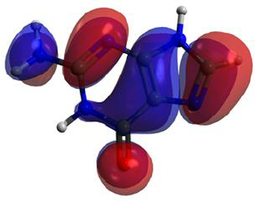
\includegraphics[width=\textwidth]{chapters/introduction/image/vbaDNA.png}
    \small\emph{Valence anion}
  \end{minipage}
  \hfill
  \begin{minipage}[b]{0.30\textwidth}
    \centering
    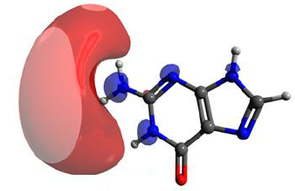
\includegraphics[width=\textwidth]{chapters/introduction/image/dbaDNA.png}
    \small\emph{Dipole-bound anion}
  \end{minipage}
  \hfill
  \begin{minipage}[b]{0.27\textwidth}
    \centering
    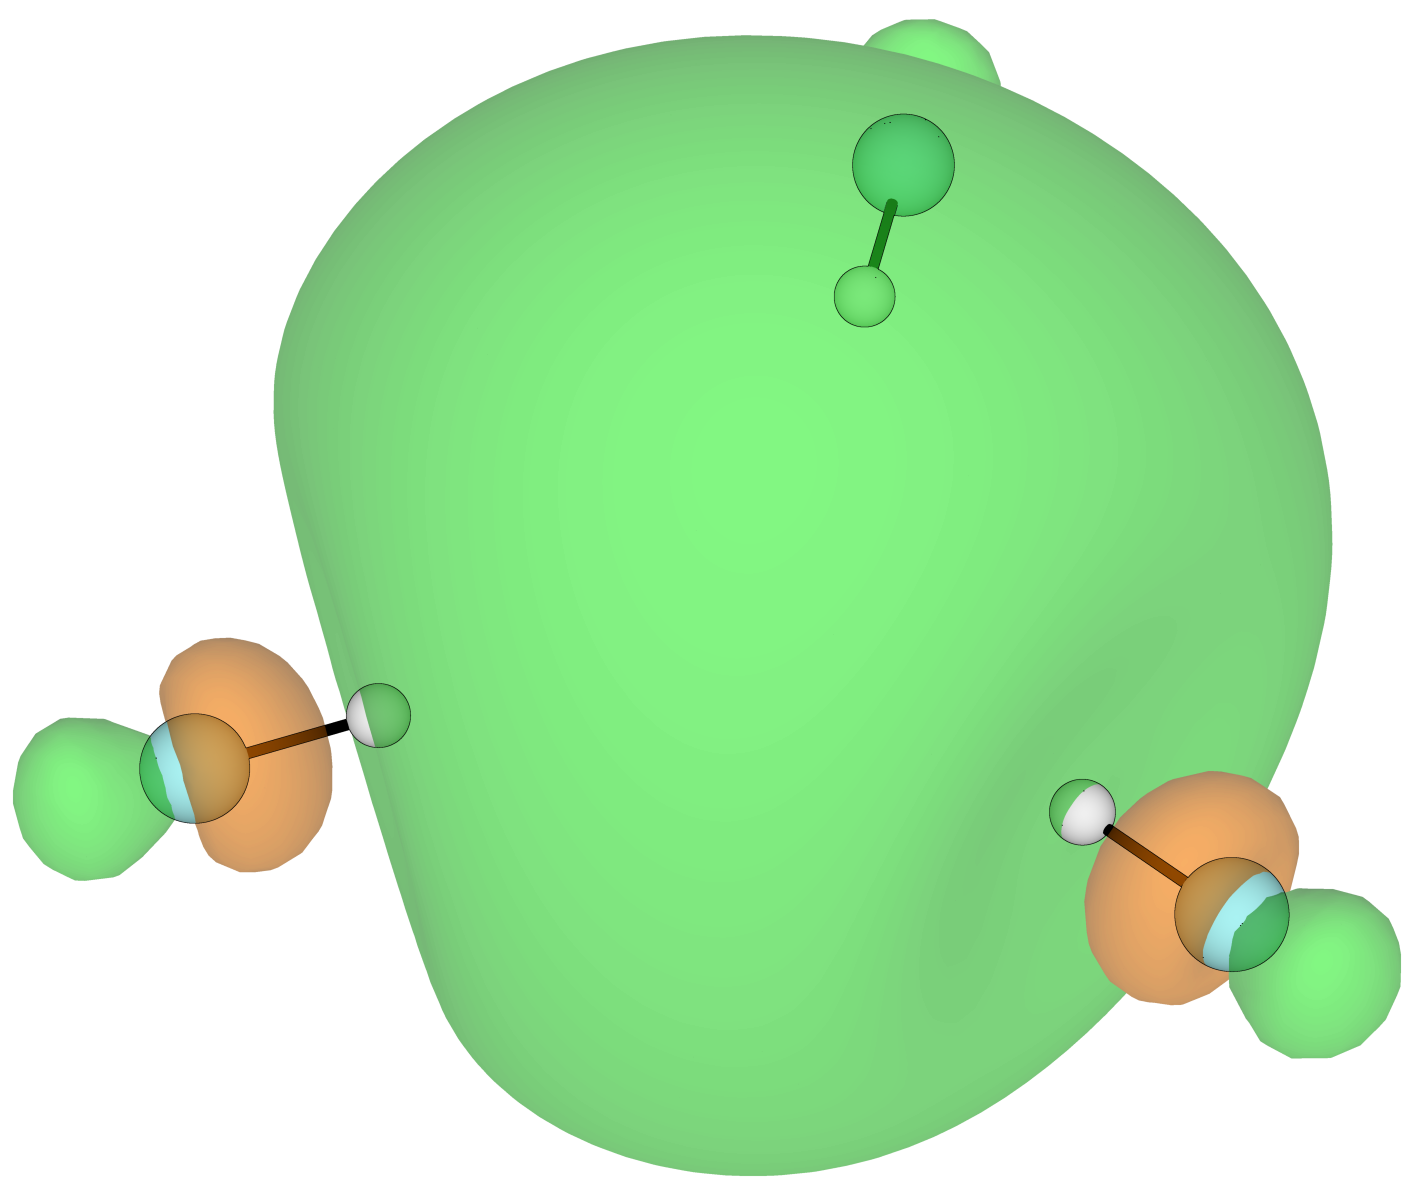
\includegraphics[width=\textwidth]{chapters/introduction/image/hf3.png}
    \small\emph{(HF)\textsubscript{3} solvated electron}
  \end{minipage}
  \caption[Valence and Non-Valence Anions]{Valence and Non-Valence Anions, a) and b) are reproduced from \cite{dutta2015electron}, c) from \cite{jordan2003theory}. \textbf{I will substitute by my own figs}}
  \label{fig:AnionTypes}
\end{figure}

\subsection{Dipole-Bound Anions}
Of the non-valence anions, dipole-bound anions (DBAs) are the most common and well-studied. Fermi and Teller first proposed the theoretical framework for non-valence bound states in 1947, demonstrating that a dipole could bind an excess electron if the dipole moment exceeds 1.625 D \cite{fermi1947capture}. Further investigations refined this concept for "real" molecules, leading to a critical dipole moment of approximately 2.5 D \cite{jordan2003theory}.

The "weak" forces that bind the excess electron are responsible for the diffusive nature of the associated orbitals, often extending several Å from the neutral molecule, and their relatively low energy, usually below 0.1 eV. This makes them susceptible to external perturbations, such as solvent interactions or external electric fields, which can significantly influence their stability and reactivity \cite{simons2008molecular,herbert2015quantum,jordan2003theory}.

Given that DBAs are bound with an energy comparable to thermal energy ($k_bT\,\sim\,23$ meV), they may seem a theoretical curiosity with limited practical relevance, destined to undergo rapid autodetachment. However, some systems can undergo a nonadiabatic transition to a stable valence anion state \cite{herbert2015quantum,jordan2003theory}. In this sense, DBSs act as "doorway" states for electron capture and transfer processes \cite{sommerfeld2002coupling,jordan2003theory,kang2024reaction}. This behaviour has spurred interest in diverse fields from astrochemistry \cite{fortenberry2015interstellar} to radiation biology \cite{narayanan2023secondary,sedmidubska2024interaction}.

\subsection{Approaches to Study Non-Valence Anions}
Significant progress has been made in experimental and theoretical methodologies for elucidating the structure and dynamics of NVAs. Experimentally, dipole-bound anions are characterised using spectroscopic and mass spectrometric techniques designed to probe their weakly bound electronic states \cite{simons2008molecular}. In photodetachment and photoelectron spectroscopies, a beam of anions is generated—often using a laser vaporisation or electrospray source—and intersected with a photon beam. The energy of the ejected electrons reveals information about the electron binding energy and electronic structure. Time-resolved photoelectron spectroscopy (TRPES) extends this approach, using ultrafast laser pulses to investigate the dynamics of electron attachment and detachment on femtosecond timescales, revealing transient states and relaxation pathways \cite{clarke2024dynamics}. DBS can also be accessed by Rydberg electron transfer spectroscopy, which has been used to probe their role in electron transfer dynamics \cite{bradforth2002excited}. Time-of-flight mass spectrometry is often coupled with these techniques to identify and isolate the correct anionic species.

The theoretical investigation of DBAs presents two main challenges. Firstly, the large spatial extent of the DB orbital requires atomic orbital basis sets that are sufficiently diffuse to accurately describe it, necessitating the use of custom basis sets \cite{skurski2000choose}. Secondly, electron correlation is important; although the electron in the DB orbital resides predominantly far from the precursor's valence electrons, the DB orbital is considerably polarisable due to its diffuse nature and exhibits significant dispersion-like interactions with the other valence electrons, contributing substantially to its binding energy \cite{simons2008molecular,simons2023molecular,gutowski1996contribution}.

Regarding computational methods, standard density functional theory (DFT) approaches can fail due to their inadequate treatment of the highly diffuse electron density and can suffer from spin contamination in open-shell systems, requiring careful selection of the exchange-correlation functional \cite{thiam2023accurately}. Multiconfigurational methods like complete active space self-consistent field (CASSCF) can address the multiconfigurational nature of these systems, but require considerable expertise in selecting an appropriate active space that balances accuracy and computational feasibility. Currently, equation-of-motion coupled-cluster (EOM-CC) methods represent the standard for DBA modelling as they adequately capture both electron correlation effects and open-shell character. However, the high computational cost of EOM-CC approaches significantly limits their applicability to larger molecular systems \cite{herbert2015quantum,jordan2003theory}. To address this, some approximate methods have been developed, such as the second order approximate CC \cite{christiansen1995second}- which is used in this work, or the domain-based pair natural implementation (DLPNO) method \cite{haldar2020multilayer}.

\subsection{Non-Valence Anions In Condensed Matter}

Several studies have indicated that the presence of individual molecules interacting with a molecule supporting an NVA can further stabilise the state by strengthening the total dipole moment, or by combining individual moments to form a "cavity" where the electron resides. The excess electron is stabilised by the collective interaction with multiple solvent molecules, rather than binding to any individual molecule, and is known as a solvated electron \cite{jordan2003theory,herbert2015quantum,jalbout2001dipole,clarke2025role}. The binding energy of such solvated electrons can increase dramatically with cluster size; while a water dimer anion (H\textsubscript{2}O)\textsubscript{2}\textsuperscript{-} exhibits a very weak vertical detachment energy (VDE) of only 0.045 eV, water cluster anions (H\textsubscript{2}O)\textsubscript{n}\textsuperscript{-} with approximately 80--100 molecules can achieve VDEs exceeding 2.0 eV. A weakly bound non-valence state transforms into a strongly bound electronic species with significantly altered properties \cite{herbert2015quantum}. In bulk, the hydrated electron is bound at 2.2 eV \cite{jordan2003theory,herbert2017hydrated}. The structure of the state was subject of much debate in the literature \cite{herbert2017hydrated,jordan2003theory}, but it is now generally accepted that the excess electron resides in a cavity of approximately 2.5 \r{A} in size \cite{herbert2017hydrated}.

In solution, the existence of a hydrated DBA is still debated \cite{anusiewicz2020fate,castellani2019stability}. The survival of NBS in condensed matter remains a subject of discussion. Computational studies suggest that hydration influences the localisation of the excess electron, often displacing it onto the solvent cage's surface \cite{anusiewicz2020fate}. Conversely, experimental evidence indicates that alkyl chains do not disrupt DBS stability \cite{castellani2019stability}, and DBS-mediated mechanisms have been observed in solvated uracil systems \cite{narayanan2024electron}. The viability of NBS in bulk systems depends on the molecular density and polarity of the medium. While solvents may hinder DBS existence due to excluded volume effects, they also stabilise DBS through Van der Waals interactions \cite{bradforth2002excited,chen2000precursors}. Distinct scenarios can be considered in the interaction between a DBA supporting molecule and solvent: the electron may be localised in the NVA orbital, captured by the solvent to form a cage, or interact with solvent molecules whose instantaneous dipole orientations stabilise the DB state. The latter two phenomena are linked to charge-transfer-to-solvent (CTTS) electronic transitions and are observed experimentally \cite{simons2023molecular,bradforth2002excited,chen2000precursors}.

\subsection{Non-Valence Anions in Biological Systems}
Expand this section explaining more about the DNA and radiosensitizers. End with some sentences about the experimants w quinones.
Research on DBAs has predominantly focused on gas-phase systems. In biological contexts, DBAs have been studied for their interactions with DNA, particularly in radiation damage and radiosensitisation \cite{gu2012interactions,narayanan2023secondary,sedmidubska2024interaction}.

Studies on electron interactions with biomolecules, both in bare and hydrated states, have highlighted the significance of DBAs in biological systems. The role of NVAs in natural biological pathways outside genetic damage remains largely unexplored. Their sensitivity to environmental factors suggests potential applications in regulating long-range electron transfer processes. It has been suggested that in proteins, vacant pockets could accommodate non-valence states \cite{castellani2019stability}.\\
\textbf{expand this section with electron transfer in proteins and more discussion?}
Most studies related to the biological importance of these NVAs are done in relation to DNA. In this study, we aim to focus on other biological targets, which could use an interplay between NVAs and valence bound electrons. A compound that is ubiquitous in nature and whose structure is interesting to study is ubiquinone.

\iffalse DBAs have been used as the explanaiton for the presence of methil functional groups electron of flavins \cite{matthews2018observation}; they would disrupt that state, making the \fi

\section{Biological Quinones}
Quinones, first isolated from the bark of the cinchona tree in the 18th century \cite{rusell1873quinone}, are a class of organic compounds with a fully conjugated cyclic dione structure derived from aromatic compounds by conversion of an even number of C-H groups into carbonyl (ketone) C=O groups \cite{IUPACQ050152025}. Quinones are known for their redox properties and play crucial roles in various biological processes, including electron transport in cellular respiration and photosynthesis \cite{ernster1995biochemical,chen2024low}.

This work focuses on ubiquinone -\textit{ubi} from being ubiquitous in nature-, also known as coenzyme Q\textsubscript{10} (CoQ\textsubscript{10}), a lipid-soluble molecule that exists as a quinone or quinol, then named ubiquinol. It plays a role in aerobic respiration in the electron transport chain (ETC) as an electron carrier, accepting 2 electrons at complexes I and II and donating them in complex III \cite{ernster1995biochemical}. CoQ\textsubscript{10}.

\begin{figure}[hb!]
  \centering
  \begin{tikzpicture}[x=1pt,y=1pt]
    \node at (140,0) {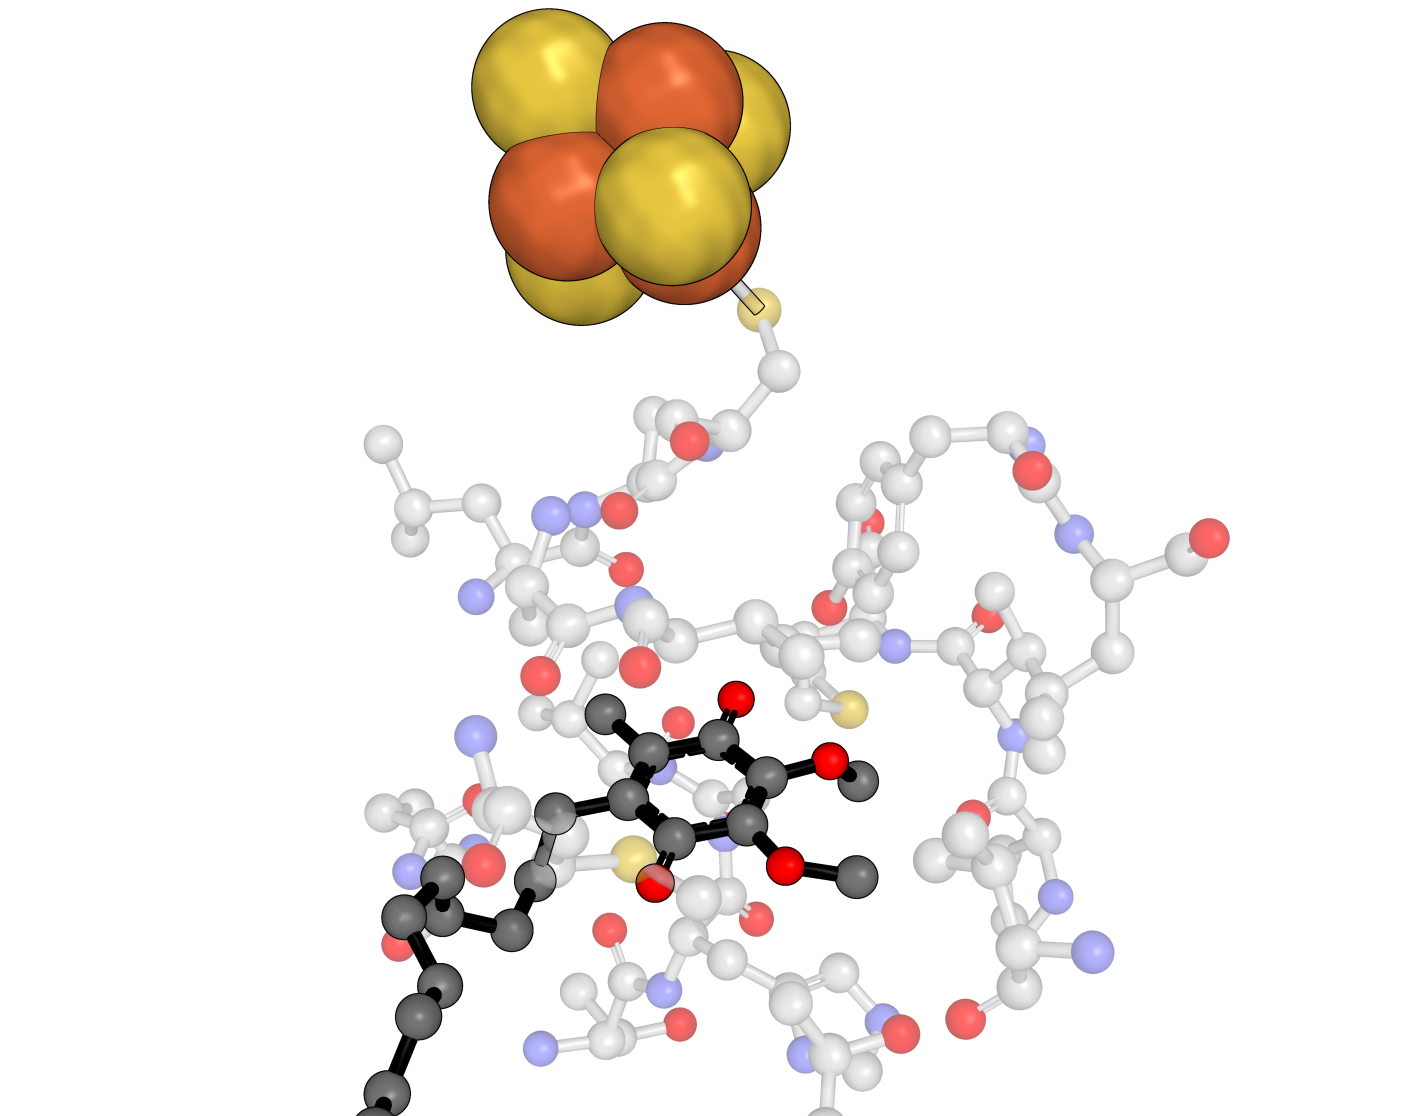
\includegraphics[width=0.45\textwidth]{chapters/introduction/image/uQ_6i0d.png}};
    \node at (215,40) {\includegraphics[width=0.25\textwidth]{chapters/introduction/image/Ubiquinone–ubiquinol_conversion.svg.png}};
    \node at (0,0) {\includegraphics[width=0.45\textwidth]{chapters/introduction/image/Mitochondrial_electron_transport_chain—Etc4.svg.png}};
    %\node[anchor=west] at (80,-225) {\fontsize{4.5}{4}\selectfont\color{darkgray}Ref: Wikimedia Commons};
    %\node[anchor=west] at (238,-285) {\fontsize{4.5}{4}\selectfont\color{darkgray}PDB: 6i0d};
  \end{tikzpicture}
  \caption[Role of ubiquinone]{\textbf{Role of ubiquinone. I will fix later}}
  \label{fig:QuinoneTypes}
\end{figure}

\subsection{Structural Aspects of Ubiquinone}
Ubiquinone is composed of a benzoquinone ring and a long isoprenoid side chain, which varies in length depending on the organism. The number of isprenoid units is the \textit{n} in the Q\textsubscript{n} scheme. The benzoquinone moiety is responsible for its redox properties, while the isoprenoid tail enhances its lipid solubility, allowing it to integrate into biological membranes \cite{ernster1995biochemical}. The benzoquinone moiety consists of 2,3-dimethoxy-6-methyl-p-benzoquinone \cite{ernster1995biochemical}.

\begin{figure}[h]
  \centering
  \begin{tikzpicture}[anchor=south west, x=1cm, y=1cm]
    \node (img1) at (0,0) {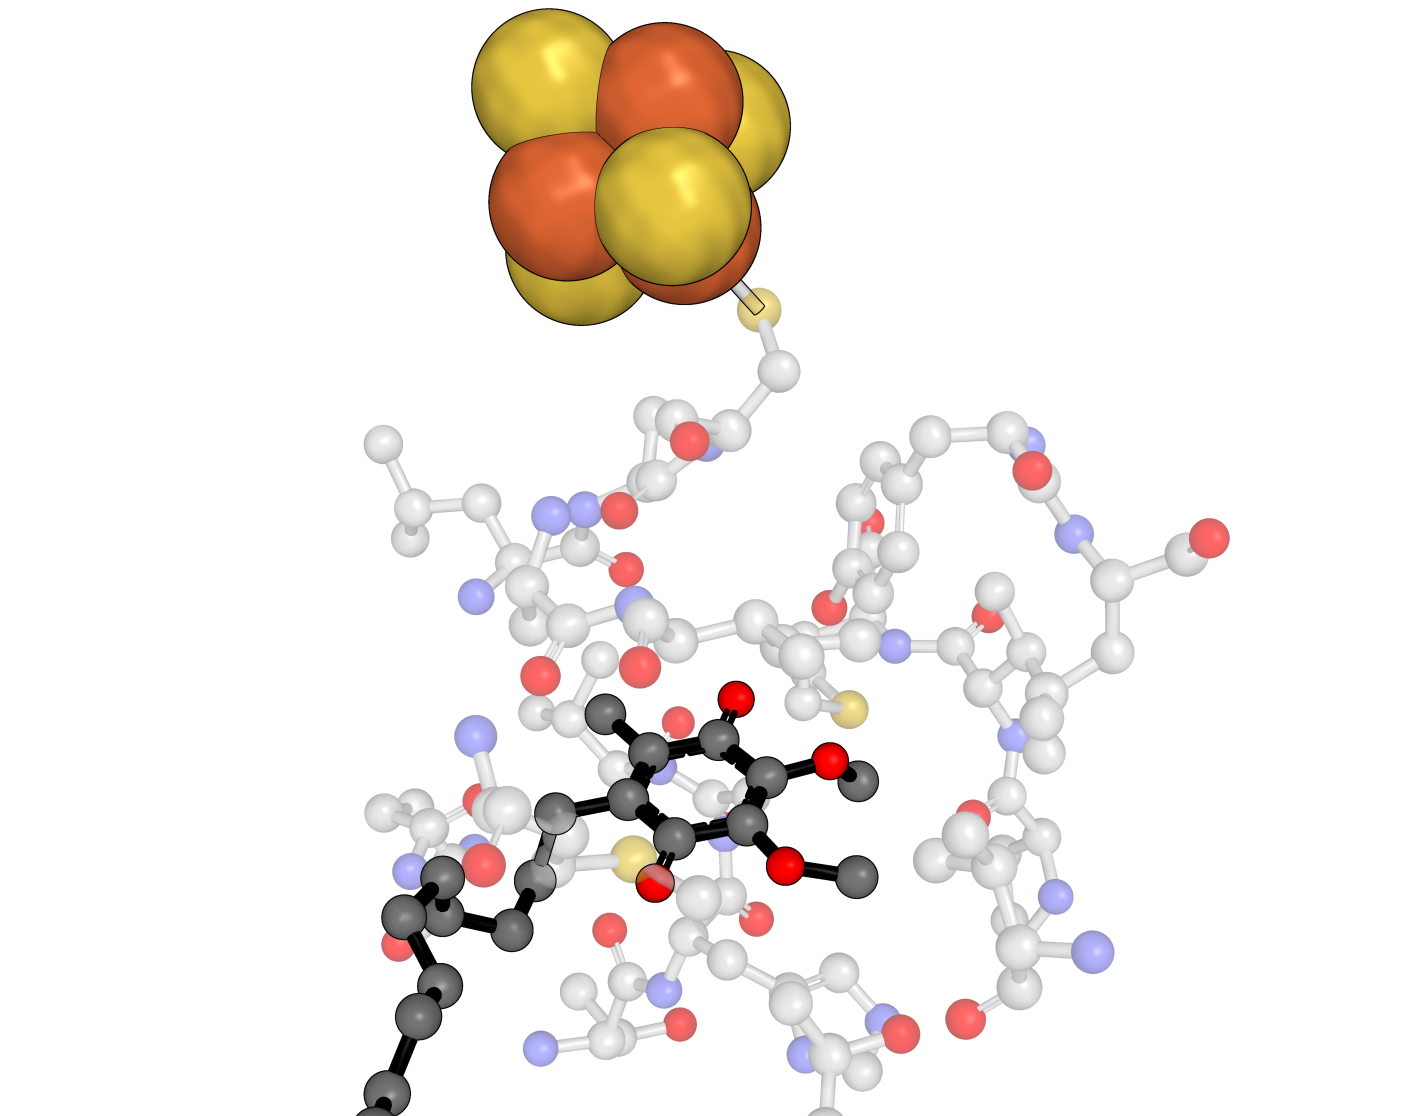
\includegraphics[width=0.4\textwidth]{chapters/introduction/image/uQ_6i0d.png}};
    \node (img2) at (0.33\textwidth,0) {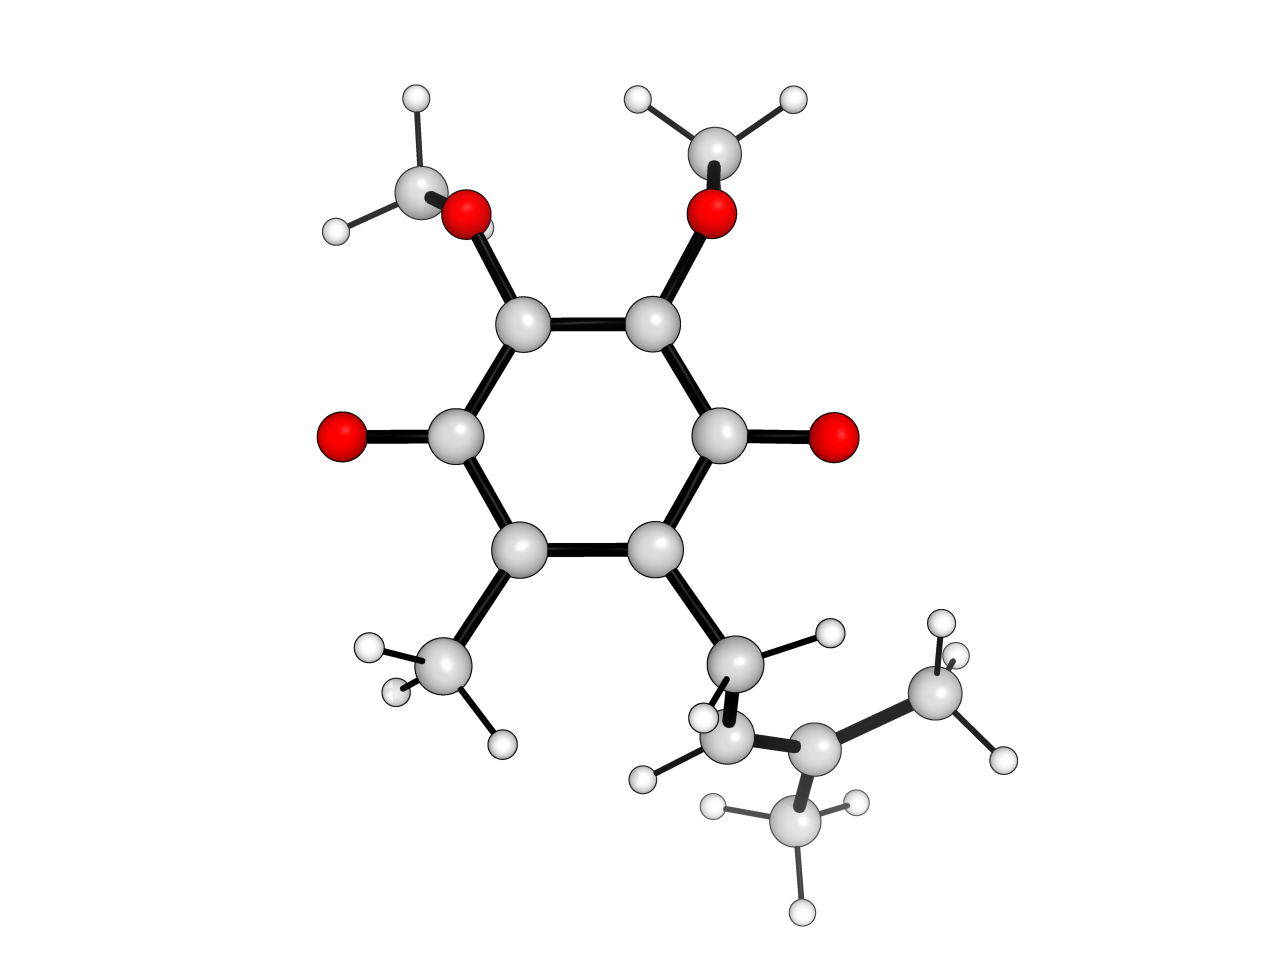
\includegraphics[width=0.4\textwidth]{chapters/introduction/image/Q1.png}};
    \node (img3) at (0.66\textwidth,0) {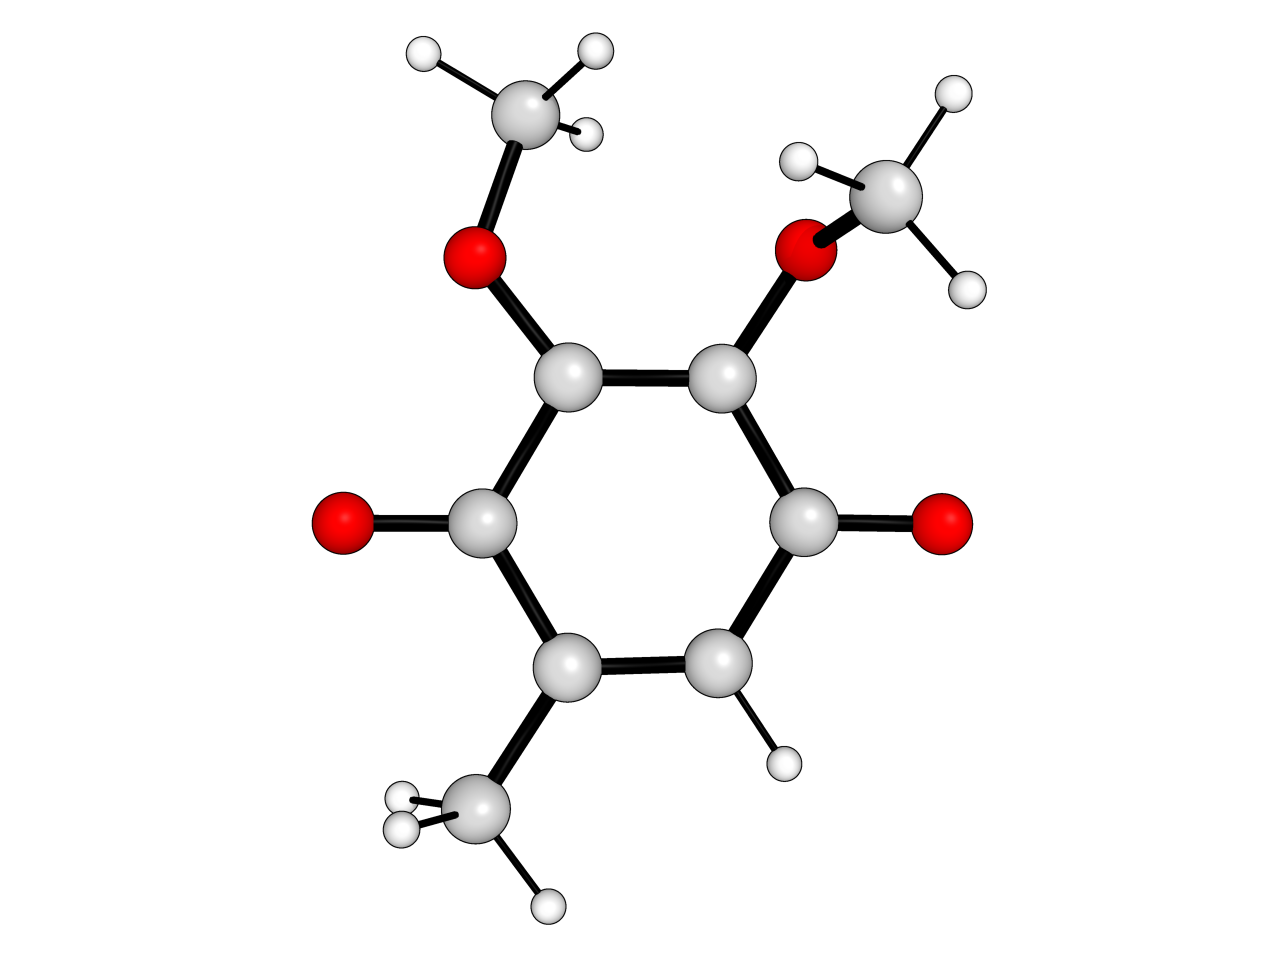
\includegraphics[width=0.4\textwidth]{chapters/introduction/image/Q0189.png}};
    \node[align=center, text=darkgray] at ([yshift=-0.8cm, xshift=-1.2cm]img1.south) {\footnotesize Q10, Cluster Model};
    \node[align=center, text=darkgray] at ([yshift=-0.8cm]img2.south) {\footnotesize Q1};
    \node[align=center, text=darkgray] at ([yshift=-0.8cm]img3.south) {\footnotesize Q0};
  \end{tikzpicture}
  \caption[Quinone structures]{Quinones used in this work. From left to right: (a) Q\textsubscript{0}, (b) Q\textsubscript{1}, (c) Q\textsubscript{10} in the enzyme PDB bla bla.}
  \label{fig:QuinoneTypes}
\end{figure}

As stated, the quinone moiety is responsible for its electron binding properties; it supports two anion states, a valence anion and a dipole bound anion. The valence anion can be understood as the equivalent state to the parent molecule, p-benzoquinone, with the excess electron located in a \textpi \textsuperscript{*} orbital. The electron withdrawing ketone groups contribute to stabilise this state, which is bound in the range of 1.7 eV \cite{chen2024low}. The dipole-bound anion, on the other hand, results mainly from the two methoxy chains, whose configuration mainly controls the dipole of the molecule \cite{ameixa2023parent}. The interplay between these groups, especially in the case of Q\textsubscript{0} - without any isoprenoid molecule, makes it a very interesting system to study theoretically. It is a fairly rigid molecule, except for the dihedral angles between the methoxy groups and the benzoquinone ring, which can be used to control the dipole moment of the molecule. This makes the study of a fairly complicated electronic structure in terms of two coordinates.

When the isoprenoid tail is considered, it has been shown that it further stabilises the valence anion \cite{pshenichnyuk2020ionizing}. Regarding its effects on the dipole state, one can imagine the effect to be moderate; it will slightly modify the dipole moment of the system, but structurally it will be quite far from the orbital occupied by the excess electron.

There have been extensive studies on the electron binding properties of the ubiquinone family, both experimentally \cite{ameixa2023parent,west2014anion,pshenichnyuk2020ionizing,bull2015anion} and theoretically \cite{ameixa2023parent,pshenichnyuk2020ionizing,haldar2020multilayer, nonella1998quantum, gamiz2017terminal}. However, these studies have been centred on understanding the valence anion of the quinone, and no comprehensive study of its dipole bound state has been performed; the VBA is the final acceptor of the electron and the existence of the DBA in condensed phase is dubious.
However, experimental studies have observed dipole-bound anions in the gas phase in ubiquinones Q\textsubscript{0} and Q\textsubscript{1} \cite{ameixa2023parent} with an EA of $\mathrm{\sim}$60 meV. Although its signal is reduced as more isoprenoid units are added, interpreted as an effect of the isprenoid tail being flexible and resulting in a steric hindrance of the state \cite{ameixa2023parent,pshenichnyuk2020ionizing}, one could imagine that in a protein moiety, the geometry of the tail would be fixed far from a potential DB orbital, which could even be further stabilised by residues pointing in the cavity.

\section{Research Objectives}
The main objective of this work is to study the dipole-bound anion of ubiquinone. The specific objectives are:
\begin{itemize}
  \item Benchmark the effectiveness of the CC2 method to model quinones electron attachment.
  \item To investigate the dipole-bound anion of ubiquinone as a function of its methoxy groups, and the effect of the isoprenoid tail.
  \item To study the effect of the protein environment on the dipole-bound anion of ubiquinone, treated as a cluster model using small molecules.
\end{itemize}

\iffalse \begin{figure}[th!]
  \centering
  % GNUPLOT: LaTeX picture with Postscript
\begingroup
  \makeatletter
  \providecommand\color[2][]{%
    \GenericError{(gnuplot) \space\space\space\@spaces}{%
      Package color not loaded in conjunction with
      terminal option `colourtext'%
    }{See the gnuplot documentation for explanation.%
    }{Either use 'blacktext' in gnuplot or load the package
      color.sty in LaTeX.}%
    \renewcommand\color[2][]{}%
  }%
  \providecommand\includegraphics[2][]{%
    \GenericError{(gnuplot) \space\space\space\@spaces}{%
      Package graphicx or graphics not loaded%
    }{See the gnuplot documentation for explanation.%
    }{The gnuplot epslatex terminal needs graphicx.sty or graphics.sty.}%
    \renewcommand\includegraphics[2][]{}%
  }%
  \providecommand\rotatebox[2]{#2}%
  \@ifundefined{ifGPcolor}{%
    \newif\ifGPcolor
    \GPcolortrue
  }{}%
  \@ifundefined{ifGPblacktext}{%
    \newif\ifGPblacktext
    \GPblacktexttrue
  }{}%
  % define a \g@addto@macro without @ in the name:
  \let\gplgaddtomacro\g@addto@macro
  % define empty templates for all commands taking text:
  \gdef\gplbacktext{}%
  \gdef\gplfronttext{}%
  \makeatother
  \ifGPblacktext
    % no textcolor at all
    \def\colorrgb#1{}%
    \def\colorgray#1{}%
  \else
    % gray or color?
    \ifGPcolor
      \def\colorrgb#1{\color[rgb]{#1}}%
      \def\colorgray#1{\color[gray]{#1}}%
      \expandafter\def\csname LTw\endcsname{\color{white}}%
      \expandafter\def\csname LTb\endcsname{\color{black}}%
      \expandafter\def\csname LTa\endcsname{\color{black}}%
      \expandafter\def\csname LT0\endcsname{\color[rgb]{1,0,0}}%
      \expandafter\def\csname LT1\endcsname{\color[rgb]{0,1,0}}%
      \expandafter\def\csname LT2\endcsname{\color[rgb]{0,0,1}}%
      \expandafter\def\csname LT3\endcsname{\color[rgb]{1,0,1}}%
      \expandafter\def\csname LT4\endcsname{\color[rgb]{0,1,1}}%
      \expandafter\def\csname LT5\endcsname{\color[rgb]{1,1,0}}%
      \expandafter\def\csname LT6\endcsname{\color[rgb]{0,0,0}}%
      \expandafter\def\csname LT7\endcsname{\color[rgb]{1,0.3,0}}%
      \expandafter\def\csname LT8\endcsname{\color[rgb]{0.5,0.5,0.5}}%
    \else
      % gray
      \def\colorrgb#1{\color{black}}%
      \def\colorgray#1{\color[gray]{#1}}%
      \expandafter\def\csname LTw\endcsname{\color{white}}%
      \expandafter\def\csname LTb\endcsname{\color{black}}%
      \expandafter\def\csname LTa\endcsname{\color{black}}%
      \expandafter\def\csname LT0\endcsname{\color{black}}%
      \expandafter\def\csname LT1\endcsname{\color{black}}%
      \expandafter\def\csname LT2\endcsname{\color{black}}%
      \expandafter\def\csname LT3\endcsname{\color{black}}%
      \expandafter\def\csname LT4\endcsname{\color{black}}%
      \expandafter\def\csname LT5\endcsname{\color{black}}%
      \expandafter\def\csname LT6\endcsname{\color{black}}%
      \expandafter\def\csname LT7\endcsname{\color{black}}%
      \expandafter\def\csname LT8\endcsname{\color{black}}%
    \fi
  \fi
    \setlength{\unitlength}{0.0500bp}%
    \ifx\gptboxheight\undefined%
      \newlength{\gptboxheight}%
      \newlength{\gptboxwidth}%
      \newsavebox{\gptboxtext}%
    \fi%
    \setlength{\fboxrule}{0.5pt}%
    \setlength{\fboxsep}{1pt}%
    \definecolor{tbcol}{rgb}{1,1,1}%
\begin{picture}(4600.00,4320.00)%
    \gplgaddtomacro\gplbacktext{%
      \csname LTb\endcsname%%
      \put(714,562){\makebox(0,0)[r]{\strut{}$-1.5$}}%
      \csname LTb\endcsname%%
      \put(714,1156){\makebox(0,0)[r]{\strut{}$-1$}}%
      \csname LTb\endcsname%%
      \put(714,1749){\makebox(0,0)[r]{\strut{}$-0.5$}}%
      \csname LTb\endcsname%%
      \put(714,2343){\makebox(0,0)[r]{\strut{}$0$}}%
      \csname LTb\endcsname%%
      \put(714,2936){\makebox(0,0)[r]{\strut{}$0.5$}}%
      \csname LTb\endcsname%%
      \put(714,3530){\makebox(0,0)[r]{\strut{}$1$}}%
      \csname LTb\endcsname%%
      \put(714,4124){\makebox(0,0)[r]{\strut{}$1.5$}}%
      \csname LTb\endcsname%%
      \put(812,386){\makebox(0,0){\strut{}$-10$}}%
      \csname LTb\endcsname%%
      \put(1680,386){\makebox(0,0){\strut{}$-5$}}%
      \csname LTb\endcsname%%
      \put(2549,386){\makebox(0,0){\strut{}$0$}}%
      \csname LTb\endcsname%%
      \put(3417,386){\makebox(0,0){\strut{}$5$}}%
      \csname LTb\endcsname%%
      \put(4286,386){\makebox(0,0){\strut{}$10$}}%
    }%
    \gplgaddtomacro\gplfronttext{%
      \csname LTb\endcsname%%
      \put(3530,3965){\makebox(0,0)[r]{\strut{}$\sin(x)$}}%
      \csname LTb\endcsname%%
      \put(3530,3789){\makebox(0,0)[r]{\strut{}$\cos(x)$}}%
      \csname LTb\endcsname%%
      \put(3530,3613){\makebox(0,0)[r]{\strut{}$\tan(x)$}}%
      \csname LTb\endcsname%%
      \put(161,2343){\rotatebox{-270.00}{\makebox(0,0){\strut{}$y$}}}%
      \csname LTb\endcsname%%
      \put(2549,123){\makebox(0,0){\strut{}$x$}}%
    }%
    \gplbacktext
    \put(0,0){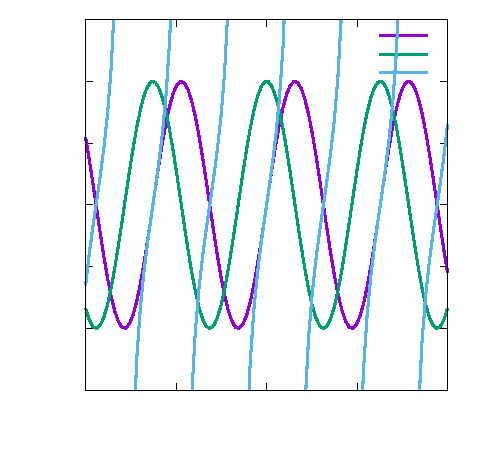
\includegraphics[width={230.00bp},height={216.00bp}]{test}}%
    \gplfronttext
  \end{picture}%
\endgroup

  %figsize is set in image/test.gp 
  \caption[Short caption for Table of Figures]{Illustration of how to
  include a figure (long text, should not go to Table of Figures).}
  \label{fig:test}
\end{figure} \fi

%%%%%%%%%%%%%%%%%%%%%%%%%%%%%%%%%%%%%%%%%%%%%%%%%%
% Keep the following \cleardoublepage at the end of this file, 
% otherwise \includeonly includes empty pages.
\cleardoublepage

% vim: tw=70 nocindent expandtab foldmethod=marker foldmarker={{{}{,}{}}}
